\documentclass[../main.tex]{subfiles}
\graphicspath{{\subfix{../images/}}}
\begin{document}

\section{Úvod}

\subsection{Značení}


$\Omega \subset \mathbb{R}^n$ omezená oblast

$\partial\Omega$ Liepschitzovská oblast - lze pokrýt konečně mnoha grafy Liepschitzovských zobrazení ($|\phi(x) -  \phi(y)| < L ||x-y||$)

$\bar{\Omega}$ - uzávěr oblasti $\Omega$

$\mathcal{C}^{(k)}(\Omega)$ spojité funkce s derivacemi do k-tého řádu spojité na $\Omega$

$\mathcal{C}^{(\infty)}(\Omega)$ hladké funkce na $\Omega$


$\mathcal{C}^{(\infty)}_0(\Omega)$ hladké funkce na $\Omega$ s kompaktním nosičem


$f\in\continuous{k}, \frac{\partial^{|\alpha|}}{\partial^{\alpha_1}x_1\partial^{\alpha_2}x_2...\partial^{\alpha_n}x_n} f = \mathcal{D}^\alpha, \alpha = [\alpha_1, \alpha_2, ..., \alpha_n], |\alpha|=\sum_i \alpha_i $




Lebesgueovy prostory
$\mathbb{L}_p(\Omega) = \{f: \Omega \mapsto \mathbb{R}| \text{měritelné}, \int_{\Omega}|f(x)|^p dx < +\infty \}$
$p \in <1, +\infty)$

$\mathbb{L}_\infty(\Omega) = \{  f:\Omega\mapsto\mathbb{R} | \text{měřitelné}, (\exists K > 0)(s.v. x \in\Omega)(|f(x)| \leq K)  \}$


\subsection{Vztahy}

\subsubsection{Minkowskeho nerovnost}
\begin{equation}\label{eq:Mink}
    \left ( \int_\Omega |f(x) + g(x)|^p dx \right ) ^{\frac{1}{p}} \leq \left ( \int_\Omega |f(x)|^p dx \right ) ^{\frac{1}{p}} + \left ( \int_\Omega |g(x)|^p dx \right ) ^{\frac{1}{p}}
\end{equation}


\subsubsection{Holderova nerovnost}
$\left (  \frac{1}{p} + \frac{1}{q} = 1 \right ), f \in \mathbb{L}_p(\Omega), g \in \mathbb{L}_q(\Omega)$
\begin{equation}\label{eq:Holder}
    \int_\Omega \left| f(x)g(x) \right| dx \leq \left ( \int_\Omega |f(x)|^p dx \right ) ^{\frac{1}{p}} * \left ( \int_\Omega |g(x)|^q dx \right ) ^{\frac{1}{q}}
\end{equation}

Dále platí:

$p_2 > p_1 \geq 1 \implies \mathbb{L}_{p_2}(\Omega) \subset \mathbb{L}_{p_1}(\Omega)$

\begin{equation*}
    \int_\Omega |f(x)|^{p_1}dx \leq \text{Holder \eqref{eq:Holder}} \leq \left ( \int_\Omega \left ( |f(x)|^{p_1}\right )^{\frac{p_1}{p_2}} \right )^\frac{p_1}{p_2} * \left ( \int_\Omega 1 ^q dx \right ) ^ \frac{1}{q}
\end{equation*}

\begin{equation*}
    \int_\Omega |f(x)|^{p_1}dx \leq \left( \int_\Omega |f(x)|^{p_2} \right)^{\frac{p_1}{p_2}} * |\Omega|
\end{equation*}

\begin{equation*}
    \int_\Omega |f(x)|^{p_1}dx \leq |\Omega| \int_\Omega |f(x)|^{p_2}
\end{equation*}




\subsection{Sobolevovy prostory }

$\mathbb{D} = \continuous{\infty}$

norma:
$||u||_{W_p^{(k)}(\Omega)} = \sum_{|\alpha| \leq K} ||D^\alpha u||_{\mathbb{L}_p(\Omega)}$

normovaný prostor: $S^{(k)}_p(\Omega) = (\mathbb{D}; ||.||_{V_p^{(k)}(\Omega)})$

Tento prostor není úplný, proto použijeme standartní zúplňovací proceduru a dostaneme:
$\mathbb{W}_p^{(k)}(\Omega)$

Obdobně můžeme postupovat pro $\mathbb{D} = \mathcal{C}^{(\infty)}_0(\Omega)$ a dostaneme $\mathbb{W}_p^{0 (k)}(\Omega)$

\subsection{Věta o stopách}

$\Omega$ - omezená oblast, $\partial \Omega$ - Liepschitzovská

$\exists_1 T: \mathbb{W}_2^{(1)}(\Omega) \mapsto \mathbb{L}_p (\partial \Omega), \text{omezený lineární operátor tak, že}$

$ \forall f\in C (\bar \Omega), Tf = f /_{\partial \Omega} $



\section{Okrajová úloha}
$\Omega\subset\mathbb{R}^n$ - omezená oblast, $\partial \Omega$ - Liepschitzovská

\begin{align}\label{eq:okraj}
    - \sum_{i,j = 1}^{n} \frac{\partial}{\partial x_i} \left ( a_{ij}(x) \frac{\partial u}{\partial x_j}\right ) + q(x)*u &= f \quad \text{v } \Omega
    \\ \label{eq:PP1}
    u|_{\Gamma_0} &= g_0 \quad \text{na } \Gamma_0 \quad \text{(Dirichletova část)}
    \\ \label{eq:PP2}
    \sum_{i,j=1}^{n}a_{ij} (x) \frac{\partial u}{\partial x_j} |_{\Gamma_1} &= g_1 \quad \text{na } \Gamma_1 \quad \text{(Neumannova část)}
\end{align}

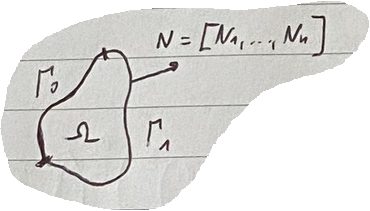
\includegraphics{images/oblast.PNG}

\subsection{Výchozí vlastnosti}
$f, g \in \mathcal{C}(\bar{\Omega})$

$a_{ij} \in \continuous[\bar{\Omega}]{1}$

$g_{0,1} \ in \mathcal{C}(\partial\Omega)$

\subsection{Silně eliptický operátor}
$(\exists C_0 > 0)(\forall \xi \in \mathbb{R}^n) (\forall x \in \Omega) (\sum_{i,j =1}^{n} a_{ij}(x)\xi^i \xi^j \geq c_0 \sum_{i = 1}^{n}|\xi^i|^2)$


Klasické řešení \eqref{eq:okraj} je funkce $u\in\continuous[\bar{\Omega}]{2}$ splňující \eqref{eq:okraj} bodově. 

\subsection{Slabá formulace}
Vezmeme \eqref{eq:okraj} a +- ji přenásobíme testovací funkcí 

Nechť $i\in \closedcontinuous{2}, v\in\closedcontinuous{\infty}, v|_{\Gamma_0 = 0}$

\begin{equation}
    - \int_\Omega \sum_{i,j = 1}^{n} \frac{\partial}{\partial x_i} \left ( a_{ij}(x) \frac{\partial u}{\partial x_j}\right ) \, dx + \int_\Omega q(x)*u*v \ dx = \int_\Omega f*v \ dx 
\end{equation}
Na první člen použijeme Greenovu identitu

\begin{equation}
    - \int_\Omega \sum_{i,j = 1}^{n}a_{ij}(x) \frac{\partial u }{\partial x_j} N_i v \ dS \
    + \int_\Omega \sum_{i,j = 1}^{n}a_{ij}(x)\frac{\partial u }{\partial x_j}\frac{\partial u }{\partial x_i}\ dx \
    + \int_\Omega q(x)*u*v \ dx = \int_\Omega f*v \ dx 
\end{equation}

První člen díky \eqref{eq:PP1} a \eqref{eq:PP2} upravíme na $- \int_{\Gamma_1} g_1 v \ dS$ a pak ho přesuneme na druhou stranu. 

Dostaneme: 

\begin{equation}
    \int_\Omega \sum_{i,j = 1}^{n}a_{ij}(x)\frac{\partial u }{\partial x_j}\frac{\partial u }{\partial x_i}\ dx \
    + \int_\Omega q(x)*u*v \ dx = \int_\Omega f*v \ dx + \int_{\Gamma_1} g_1 v \ dS
\end{equation}

První část označme $a(u,v)$ a druhou $\tilde{F}(v)$

\end{document}